\documentclass[8pt, %font size
a5paper, %paper type
twoside, % two sided printing
openright, % start new chapter on right side only ( inserts blank pages )
abstract=on, % Use an abstract
DIV=11,      % This parameter organizes the borders (detailed explanation at http://texdoc.net/texmf-dist/doc/latex/koma-script/scrguide.pdf
BCOR=8mm]{scrbook} % BCOR sets the space, used by the type of  book. (e.g. glued, hard cover..)
%scrreprt is used for larger texts with chapters (Master or Bachelor Thesis)
%scrartcl is used when there are no chapters ( for smaller paper)

\usepackage{fontspec}   %加這個就可以設定字體
\usepackage{xeCJK}      %讓中英文字體分開設置
%設定中文為系統上的字型,而英文不去更動,使用原TeX字型
\setCJKmainfont[AutoFakeBold=2,AutoFakeSlant=.4]{思源宋體}
\setCJKsansfont[AutoFakeBold=2,AutoFakeSlant=.4]{Noto Sans CJK TC}
\setCJKmonofont[AutoFakeBold=2,AutoFakeSlant=.4]{Noto Sans Mono CJK TC}
\XeTeXlinebreaklocale "zh"             %這兩行一定要加,中文才能自動換行
\XeTeXlinebreakskip = 0pt plus 1pt     %這兩行一定要加,中文才能自動換行
\leftskip=0pt                          %左右對齊
\rightskip=0pt plus 0cm                %左右對齊
\defaultCJKfontfeatures{AutoFakeBold=2,AutoFakeSlant=.4} %以後不用再設定粗斜
\newCJKfontfamily\Kai{I.Ngaan}         %定義指令\Kai則切換成顏楷體
\newCJKfontfamily\Hei{思源黑體}        %定義指令\Hei則切換成思源黑體
\newCJKfontfamily\NewMing{新細明體}    %定義指令\NewMing則切換成新細明體
\newCJKfontfamily\Newsong{I.BMing}
\newCJKfontfamily\Song{思源宋體}       %定義指令\Hei則切換成思源宋體
\newCJKfontfamily\SKai{全字庫正楷體}   %定義指令\SKai則切換成全字庫正楷體

\usepackage{graphicx}
\usepackage{float}
\usepackage{wrapfig}
\setlength\intextsep{5pt}


\usepackage[utf8]{inputenc}
\usepackage[english]{babel} % sets up english hyphenation
\usepackage{csquotes} % for language-dependent quotes in biblatex
\usepackage[unicode=true]{hyperref} % enables use of metadata for pdfs and hyperlinks within a document
\usepackage[natbib,maxnames=2,maxbibnames=100,style=authoryear-comp,uniquename=full,firstinits,doi=false,backend=biber,backref,hyperref]{biblatex} % advanced bibliography support
\usepackage[usenames,dvipsnames,hyperref]{xcolor} % enables more advanced color support for hyperref
\hypersetup{colorlinks=true, %flag for prints
    hidelinks,  % this option would hide links for the print version of your thesis
    linkcolor=red!35!black,    %definition of the link color
    citecolor=green!35!black,  %definition of the cite color
    urlcolor=magenta!35!black, %definition of the url color
    %pdfauthor=, % Optional: Specify the author of the pdf
    %pdftitle=   % Optional: Specify the title within the pdf
}      
\usepackage{subfiles} %This package is used for subfiles
\usepackage{tabu}     % provides advanced tables
\usepackage{array,multirow}
\bibliography{thesis.bib}% Include all the bibliography files
\usepackage{booktabs} % enables reference bookstyle tables
\usepackage[format=plain, labelfont=bf]{caption}
\usepackage{amsmath}
\usepackage[capitalize,noabbrev]{cleveref}
\usepackage{subcaption} % enables use multiple figures in a figure
\captionsetup{compatibility=false}
\usepackage{eurosym} %includes the euro symbol 
\usepackage{enumitem} % allows customization of enumeration and itemize environment
\usepackage{graphicx} % enables loading of graphics
\usepackage{tikz} % drawing vector graphics in latex
%\usepackage{parskip} %alternatively parskip replaces paragraph indentation by increased in-betweeen-paragraph linespacing 
\usepackage{setspace} % helps setup line spacing
%\onehalfspacing % increases linespacing to one and half
\usepackage{placeins} % provides FloatBarrier
%\usepackage[miktex]{gnuplottex} % gnuplot within latex. May be obsolete with pylab.
\usepackage[ruled,vlined]{algorithm2e} %algorithm package
\linespread{1.1} % Definition of the linespread
\usepackage[tbtags]{mathtools}
\DeclareMathOperator*{\somefunc}{somefunc}

%tikz helps to draw nice pictures with a lot of effort for advanced users
\usetikzlibrary{positioning,shapes,shadows,arrows, backgrounds}
\usepackage{verbatim}
\usepackage{tikz-3dplot}


%some definitions for the cref package
\crefname{algocf}{Algorithm}{Algorithms}
\crefname{table}{Table}{Tables}
\crefname{chapter}{Chapter}{Chapters}
\crefname{equation}{Equation}{Equations}
\crefname{section}{Section}{Sections}


\tikzset{
    tri/.style={
        draw,
        shape border rotate=90,
        isosceles triangle,
        isosceles triangle apex angle=60,
        node distance=1cm,
        minimum height=4em
    }
}



\begin{document}
    \frontmatter

    \begin{titlepage}
        \begin{center}

            % Upper part of the page. The '~' is needed because \\
            % only works if a paragraph has started.
            \includegraphics{img/logo2}\\[1cm]

            \textsc{\LARGE Rheinische\\[5mm] Friedrich-Wilhelms-Universität Bonn}\\[1.5cm]

            \textsc{\Large Master thesis}\\[1.5cm]

            % Title
            { \Large \bfseries Basic \LaTeX \, Template }\\[1.4cm]

            % Author and supervisor
            \begin{minipage}[t]{0.4\textwidth}
                \begin{flushleft} \large
                    \emph{Author:}\\
                    Max \textsc{Mustermann}
                \end{flushleft}
            \end{minipage}
            \begin{minipage}[t]{0.5\textwidth}
                \begin{flushright} \large
                    \emph{First Examiner:} \\
                    Prof.~Dr.~John \textsc{Doe} \\[0.5cm]
                    \emph{Second Examiner:} \\
                    Prof.~Dr.~John~\textsc{Doe} \\[0.5cm]

                    \emph{Advisor:} \\
                    John \textsc{Doe} \\[0.5cm]
                        %\emph{Abteilung:} \\
                        %Autonome Intelligente Systeme
                \end{flushright}
            \end{minipage}

            \vfill

            % Bottom of the page
            {\large Submitted:\hspace{1cm} \today}

        \end{center}
    \end{titlepage}

    \pagestyle{headings}  % switches on printing of running heads
    \title{Basic \LaTeX \, Template}
    %\subtitle{Master thesis}
    \author{Tobias Hartmann\\ \begin{minipage}{8cm}\centering \small Friedrich-Wilhelms-Universität Bonn\\ \small (group)\end{minipage}}

    \vspace{4cm}

    \cleardoublepage
    \thispagestyle{empty}
    {\noindent%
        \huge{\textbf{\textsf{Declaration of Authorship}}}
    }
    \vspace{2cm}
    \begin{flushleft}
        \noindent%
        I declare that the work presented here is original and the result of my own investigations.
        Formulations and ideas taken from other sources are cited as such.

        It has not been submitted, either in part or whole, for a degree at this or any other university.
    \end{flushleft}

    \vspace{8cm}
    \noindent%
    \rule[1em]{8em}{0.5pt}  \hfill \rule[1em]{8em}{0.5pt}\\ % This prints a line to write the date
    Location, Date \hfill Signature\\


    \cleardoublepage


    \chapter*{Abstract}
    \thispagestyle{empty}
    Describe your approach and results shortly in the abstract.
    The abstract should really already tell the reader what to expect.
    Do not try to  build suspension, this is not a Holywood  movie, it is a
    (your!) scientific thesis.  The abstract  is usually the last thing you
    write, even if it is the first thing you read here.

    \tableofcontents
    \listoffigures
    \listofalgorithms

    \newpage
    \mainmatter
    \subfile{content/introduction}

    \chapter{Language}

    \section{I or We?}

    Use the ``we'' form, even when  you're writing alone.  Imagine it to be
    the reader and  you, who are going through the  text together.  It gets
    you closer to your audience.

    \section{Quotes and Emphasis}
    Note that double "quotes" on  your keyboard are not typeset correctly. 
    English  quotes should  look like  ``this'', while  German quotes  are 
    typeset  like \glqq this\grqq.   Note the  difference.  Some  editors 
    insert the correct quotes automatically for you.                       

    Use  emphasis  sparingly.  It  clutters  the  text.  In  general,  use 
    \emph{italics}, which is the one standing out the least.  In captions, 
    it is sometimes useful to use  \textbf{bold} for the signal words left 
    and right, top and bottom: There, you want them to pop out.

    \section{Line Noise and Colloquial Expressions}

    Do  not use  fill words  which do  not carry  meaning.  Try  to be  as 
    specific as  possible.  This does  not mean  as short as  possible, it 
    means that you should have something to say when you write something.
    If you don't know what you want to say, think again, \emph{then} write.

    Don't use colloquial expressions.  In particular, don't use any of the 
    short forms  \emph{don't, aren't,  isn't, you're, we're,  \ldots}.  Do 
    not\footnote{this is much better!} use  ellipsis (\ldots) in the text, 
    as it looks like you're trailing off.                                  

    \chapter{Comments on Writing in LaTeX}

    \section{\LaTeX{}'s Wide Margins}

    Many students  complain  about  large  \LaTeX{}  standard  margins. 
    Typographers have a  rule, though: You shouldn't have  more than about 
    70 characters  per line (when  using single spacing).   Otherwise your 
    eyes have  trouble jumping to  the beginning  of the next  line.  This 
    limits  your column  width severely,  unless you  use a  big font.   A 
    thin  column width  results in  large  margins.  This  is (aside  from 
    portability) the reason  why books are smaller than A4  paper, and why 
    newspapers have multiple thin columns.                                 

    If  you want  to toy  with margins  nevertheless, consider  this: When 
    you  open  your  double-sided  printed thesis,  the  white  region  in 
    the  left/right  and  center  region should  have  equal  widths.   It 
    follows  that outside  margins  are larger  than  the margins  inside. 
    Consequentially, on  a left page,  left margins are larger  than right 
    (i.e.\ center) margins, and on a  right page, right margins are larger 
    than the left (i.e.\ center) ones. The  margin on the bottom should be 
    larger than  on the top.   These rules  are automatically used  by the 
    KomaScript classes  (scrartcl, scrbook, scrrprt).  Do  not meddle with 
    them.                                                                  
    
    To   meddle  with   the   margins,   use  the   DIV   option  of   the 
    \verb+documentclass+  command.    Larger  values  result   in  smaller 
    margins.  If you  want to bind your thesis, make  sure to include some 
    space for  it using BCOR\@.   Ask the print shop  how much to  use for 
    your  specific binding  needs.  Never,  ever, use  the \verb+geometry+ 
    package.                                                               

    \section{Paragraphs are Empty Lines}
    \label{sec:paras}

    Paragraphs are separated  by empty lines in the  \LaTeX{} code.  Never 
    use  the double  backslash for  this purpose.   \LaTeX{} inserts  page 
    breaks  preferably between  paragraphs.  A  double backslash  lets you 
    stay in the  same paragraph, so \LaTeX{} does not  know where it would 
    be good  to insert page  breaks, figures, tables, algorithms,  and the 
    like.                                                                  

    Many  people find  the  indentation  of the  first  line in  paragraph 
    odd.  Look into  a favorite book or newspaper of  yours and you'll see 
    that this way of introducing  new paragraphs is used everywhere.  Note 
    that it  allows you---even on the  top of a new  page---to see whether 
    the line is the first of a new paragraph or the continuation of an old 
    paragraph.                                                             

    \section{Typesetting Math as Part of Your Text}

    Formulas are part of the text, try  to use them like nouns and be sure 
    to include  punctuation to  keep the text  flowing.  For  example, the 
    pythagorean theorem,                                                   
    \begin{align}
        a^2 + b^2 = c^2,
    \end{align}
    is typically taught at school.

    Other random notes:

    \begin{itemize}
        \item
    Note that  as in \cref{sec:paras},  before and after a  formula, empty 
    lines will  add space  and indentation, and  possibly page  breaks, or 
    figures.  So  if a formula  is part of a  paragraph, do not  add empty 
    lines around it in the code.                                           

        \item
    Number all equations.  It makes it  easier to refer to them for others,
    even if you do not refer to them in your own text.

        \item
    While we're at  it, do not use the  \verb+equation+ or \verb+eqnarray+ 
    environments, use \verb+align+ instead.

        \item
    Take care to always put all  math in the math-environment, for example 
    the  variable $x$.   Note  that  it is  typeset  differently from  the 
    letter~x.

        \item
    Use  single-letter  names  for  variables   in  math  (math  is  not  a
    programming language!).   Function names  may have  multiple characters,
    such as $\tanh(x)$.  Note that they are not typeset in italics.  
    They  usually have  their own  commands, and  you can  define your  own
    functions, such as  $\somefunc(x)$.  If you don't do  this, the kerning
    will  be broken,  since \LaTeX{}  assumes that  you're multiplying  the
    variables  $s$, $o$,  $m$, $e$,  $f$, $u$,  $n$, and  $c$ and  typesets
    accordingly,  compare  $somefunc$  (math  mode,  without  spaces!)  and
    \emph{somefunc} (italics).

    \end{itemize}

    \section{Referencing Sections, Figures, etc.}
    Use  the \verb+cleverref+  package to  refer  to other  places in  the 
    document,  e.g.  \cref{chap:Introduction}.    The  package  allows  to 
    specify the reference style globally.  Therefore, it helps to refer in 
    a consistent  way.  Otherwise you  may quickly have different  ways of 
    referencing,   e.g.  \emph{Figure},   \emph{figure},  \emph{Fig.}   and
    \emph{fig.}.   The package  also ensures  that there  is no  linebreak 
    before the number of the figure/chapter etc.                           

    \begin{figure}
        \centering
        \begin{subfigure}[b]{0.3\textwidth}
            \includegraphics[width=\textwidth]{img/cat.jpeg}
            \caption{Nyan cat}
            \label{fig:cat1}
        \end{subfigure}%
        ~ %add desired spacing between images, e. g. ~, \quad, \qquad, \hfill etc.
        %(or a blank line to force the subfigure onto a new line)
        \begin{subfigure}[b]{0.3\textwidth}
            \includegraphics[width=\textwidth]{img/cat.jpeg}
            \caption{Nyan cat}
            \label{fig:cat2} 
        \end{subfigure}
        ~ %add desired spacing between images, e. g. ~, \quad, \qquad, \hfill etc.
        %(or a blank line to force the subfigure onto a new line)
        \begin{subfigure}[b]{0.3\textwidth}
            \includegraphics[width=\textwidth]{img/cat.jpeg}
            \caption{Nyan cat}
            \label{fig:cat3}  
        \end{subfigure}
        \caption[Nyan cats]{Pictures of Nyan cats}\label{fig:cats}
    \end{figure}



    \section{Citing Other Works}
    There are two ways to cite, which depends on whether the authors are an
    active part of your sentence:
    \begin{itemize}[noitemsep]
        \item \citet{muster} showed that\ldots{}
        \item This is currently a hot research topic \citep{muster}
    \end{itemize}
    In  \LaTeX{}, these  different  citation styles  are  reflected in  the
    \texttt{\textbackslash citet}  and  \texttt{\textbackslash citep}  commands. \textbf{Never  use  the  plain
    \texttt{\textbackslash cite}!} -- it is outdated.
    This distinction  is even more important  when you use a  numeric style
    for referencing, where in the second version only the number of the 
    reference is printed.   In the first case, a  number-only citation does
    not make much sense.

    In  your  bibliography, you  should  define  common strings,  such  as 
    conference  names, using  the  \verb|@string|  syntax.  Otherwise  you 
    might  quickly end  up with  a  lot of  different names  for the  same 
    conference, which is confusing and  inconsistent.  (Please have a look 
    at the bibliography file.)                                             

    \section{Floats}
    \subsection{Figures}
    You should  allow \LaTeX{} to place  the figures where it  wants.  The 
    same  goes  for  tables.   This  is  called  a  \verb+float+,  as  the 
    figure/table floats around.   Look in a well-typeset  book, and you'll 
    notice that figures aren't placed randomly in the text, they're rather 
    always  on the  top  of  the page  if  at  all possible. \LaTeX{}  has 
    options to  let figures float to  \emph{top} (\verb+t+), \emph{bottom} 
    (\verb+b+),   \emph{page  of   floats}   (\verb+p+)  and   \emph{here} 
    (\verb+h+).  The  default, \verb+tbp+, is  ok for most users,  in any 
    case, never use \verb+h+.  You can use the FloatBarrier command if you 
    want to make sure that a figure is within a specific section.          

    All figures have  a caption from which you can  understand most of the 
    figure content  and its significance.   They are also  referenced from 
    the main text (e.g., see \cref{fig:cats}).  Do not force linebreaks in 
    captions.  Do not deviate from these rules, they are strict.           

    Figures  should  provide a  short  name  for  every figure  in  square 
    brackets: $[$~$]$. If  you do not define a short  name, the whole text 
    of the caption will be displayed in the table of figures, which is 
    usually too long.
    
    Note that \cref{fig:cats} also shows how to use subfigures.



    \subsection{Tables}
    Never  use vertical  lines in  tables.  See  the documentation  of the 
    booktabs  package  for  an  explanation,  or  look  in  your  favorite 
    scientific  book/magazine to  understand  that this  is a  commonplace 
    rule.                                                                  

    A basic  example, taken  from the booktabs  documentation, is  given in
    \cref{tab::ex}.

    \begin{table}
        \centering
        \begin{tabular}{@{}lrr@{}} 
            \toprule
            \multicolumn{2}{c}{Education}\\ \cmidrule{1-2}
            Major & Duration & Income (\euro)\\ 
            \midrule 
            CompSci & 2 & 12,75 \\ \addlinespace
            MST & 6 & 8,20 \\ \addlinespace
            VWL & 14 & 10,00\\ 
            \bottomrule
        \end{tabular}
        \caption[Table Example]{A basic example from the booktabs package.}
        \label{tab::ex}
    \end{table}

    \paragraph{The tabu package}
    The tabu package provides some useful tools for advanced tables.


    \subsection{Algorithms}
    There are several packages to typeset algorithms.
    We recommend the \verb+algorithm2e+ package.
    In \cref{alg:exp} a simple example from the algorithm2e documentation is given.

    \begin{algorithm}[t]
        \SetAlgoLined
        \KwData{this text}
        \KwResult{how to write algorithm with \LaTeX2e }
        initialization\;
        \While{not at end of this document}{
            read current\;
            \eIf{understand}{
                go to next section\;
                current section becomes this one\;
            }{
                go back to the beginning of current section\;
            }
        }
        \caption{How to write algorithms (Small example from the algorithm2e documentation)}
        \label{alg:exp}
    \end{algorithm}

    \section{Miscellaneous}

    \subsection{Enumerations}

    Short enumerations look ugly in  standard \LaTeX{}, since they include 
    too much  space between the  items.  A ``normal'' enumerate  list with 
    very short paragraphs:                                                 
    \begin{enumerate}
        \item foo bar baz
        \item foo bar baz
        \item foo bar baz
    \end{enumerate}

    A list using enumitem to compress the inter item spaces, looks much better for short items:
    \begin{enumerate}[noitemsep]
        \item foo bar baz
        \item foo bar baz
        \item foo bar baz
    \end{enumerate}

    \subsection{Front, Main and Back Matters}

    Titlepage, lists of figures, table of contents page etc.\ are numbered 
    in  roman letters.   The introduction  should start  with page  $1$ in 
    arabic  numerals.   The document  class  \verb+scrbook+  does this  by 
    default,  when \textbackslash  frontmatter, \textbackslash  mainmatter 
    and \textbackslash backmatter are placed properly.                     



    \section{Compiling The Document}
    \LaTeX{}  is  a bit  archaic  to  work  with,  since with  every  pass 
    through  your document,  some intermediate  information is  written to 
    files,  which are  then processed  by  other programs.   Keep in  mind 
    that  everytime a  new  pass through  your  document incorporates  new 
    information (e.g. from BibTeX), page breaks may change, which requires
    an  additional pass  through the  document. Thus, you  usually have  to
    compile the document in three steps:
    \begin{enumerate}
        \item Compile the document using xelatex: xelatex thesis
        \item Run biber  (or if  you do  not have  it, bibtex)  to set  up
              bibliography: biber thesis
        \item Run xelatex  twice more to incorporate  bibtex references and
              to get the typesetting right.
    \end{enumerate}

    If  you know  what  you're doing  you  can get  away  with less.   Some
    programs parse the  output of \LaTeX{} to  determine whether additional
    passes are necessary.  Most GUI programs fall in this category, as do
    \verb+rubber+ and \verb+latexmk+.

    \subsection{Issues With This Template}
    \begin{description}
        \item [My references can't be found] 
            The line including the \texttt{biblatex} package says it should
            use \texttt{biber} as a backend.  This is a reimplementation of
            BibTeX. If you do not have \texttt{biber}, or your IDE does not
            support it, consider switching the backend to \texttt{bibtex}.
    \end{description}
\chapter{【不多看一眼】}


\begin{wrapfigure}{r}{0.3\textwidth}
\centering
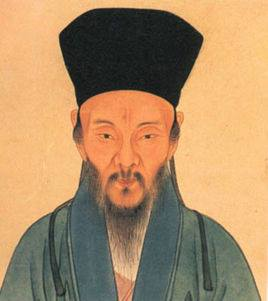
\includegraphics[width=0.3\textwidth]{pics/p001.jpg}
\vspace{-25pt}
\caption{王守仁}
%\label{test}
\end{wrapfigure}

文/喬凱凱
\footnote{摘自{\Kai《讀者》}雜誌2018年10月號與【讀者雜誌讀書會】臉書社團、【讀者雜誌粉絲團】}

12歲時,王守仁正式就讀私塾。
去私塾時,要經過一條熱鬧的大街,
街尾處有一家每天都擠滿了人的小賭坊。
見此,王守仁向同伴提議換一條路走。

「他們賭他們的,我們走我們的,互不相干,有什麼關係?」同伴很不解。

王守仁說:「我怕看多了,會產生欲望。」

同伴哈哈大笑起來:「你的意志力太不堅定了。看幾眼根本不要緊。」

同伴不以為意,堅持走原來的路線,但王守仁還是決定繞道去私塾。

後來去私塾時,偶爾會遠遠地看到同伴站在小賭坊門口,聚精會神地向裡面張望。
每當此時,王守仁便會提醒他不要靠近賭坊。
同伴擺擺手說:「只是看幾眼,沒事。」王守仁無奈,只好搖搖頭走開。

一個多月後,同伴接連幾天都沒來私塾上課。
聽其他學生說,同伴前段時間迷上了賭博,越玩越大,
甚至還偷了家裡珍藏的玉器去賭博。
他的父母得知後非常生氣,讓他在家中反省。

王守仁歎了口氣說:「想要避免沉迷於欲望,最好的辦法就是遠離,
甚至不多看一眼。這不是膽小,而是從根源上隔絕欲望。」


\chapter{【淮南王】}
\begin{wrapfigure}{r}{0.3\textwidth}
\centering
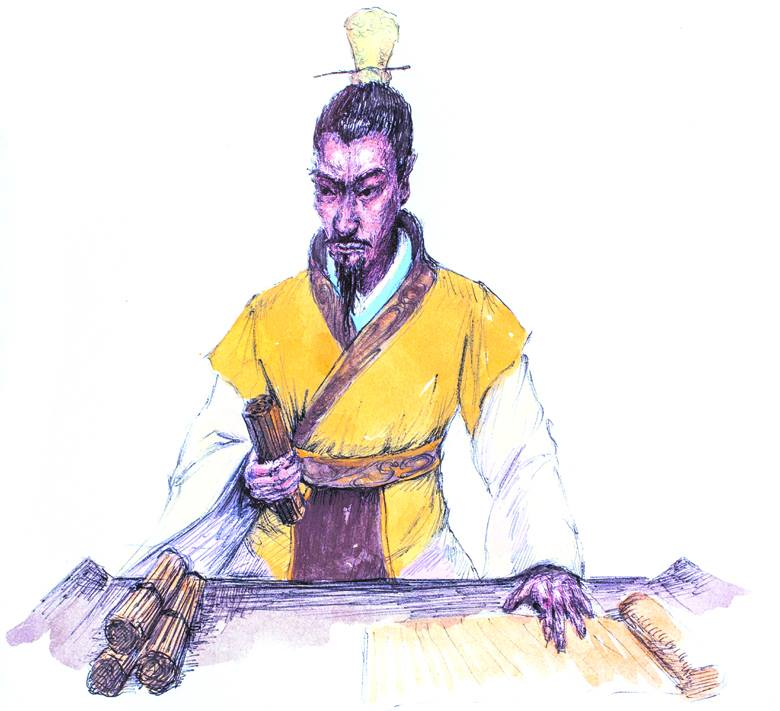
\includegraphics[width=0.3\textwidth]{pics/p002.jpg}
\vspace{-25pt}
\caption{淮南王}
%\label{test}
\end{wrapfigure}

$\cdots\cdots$ 發明豆腐 $\cdots$ 「一人得道,雞犬升天」 $\cdots\cdots$
\footnote{摘自{\Kai《讀者》}雜誌2015年11月號,圖/李發友}


讀{\Kai《史記》}如讀小說,輕鬆、好玩,而且耐人尋味。
沛縣的混混劉邦得了天下,分封諸王,異姓的倒有幾個有名的,
還都讓他給廢了,從此立個臭規矩,非劉氏不王。
可是,自家孩子封的王,大抵籍籍無名,
都是混吃等死的主兒,唯一例外的是淮南王。

第一任淮南王劉長,說起來有點來路不明。
他的母親,原是漢初異姓王趙王張敖的美人,
諸姬妾之一,後來劉邦過境,張敖為了拍劉邦的馬屁,
把美人送給劉邦侍寢。這樣的事,此前有,此後也沒斷了。

但凡款待牛人或者上司,送個美人給嘗嘗鮮,就跟送金銀玉帛一樣稀鬆平常。
牛人睡過之後,揚長而去,就當什麼事也沒發生。
這樣的美人禮物,可以送張三,也可以送李四,當然也可以自己享用。
所以,即使有了孩子,也未必能知道是誰的。那年月又沒有DNA鑒定,誰能說得清?

但是,張敖的美人,自打為劉邦侍寢之後,居然懷孕了,
而被張敖斷定為劉邦的種,不再染指,供了起來,直到生下龍子,
或者說是他認為的龍子。等到趙王張敖連同妻妾一併被劉邦找茬收了,
這件事便被有司得知,彙報上去。劉邦也不加理會,顯然是不大相信。
美人的兄弟託關係找到呂后身邊的寵臣審食其,審食其將此事告訴了呂后。
呂后當然不會喜歡劉邦身邊再多一個美女,自然一言不發,審食其當然也就只好算了。

沒想到,這個就為劉邦侍寢一次的美人,居然憤而自殺。
她這一死,讓劉邦相信了這個孩子可能真的是他留的種。
於是,劉邦就又多了一個兒子劉長。
待到原來的淮南王英布被劉邦逼得造反而被滅掉,
劉長就成了淮南王。

這個劉長,幼年喪母,卻長得很結實,力氣很大,能扛鼎,估計也喜歡舞槍弄棒的。
對他娘的死,他一直耿耿於懷。其實,他娘的死,該賴他的爹。
但那時的人怎麼敢恨自己的父親,於是就遷怒於辟陽侯審食其。

劉長長大以後,已經是漢文帝的天下了,一日,他袖裡藏著一枚鐵錘,
找上審食其的門去,光天化日之下一錘就將這位侯爺給打倒了,
然後讓人將其腦袋割下。然後,劉長大模大樣地到皇帝那兒去請罪,
說是請罪,卻說了一大串審食其的罪過。這個劉長,見了皇帝,
不稱陛下,只叫「大兄」的。這個皇帝還能把他怎麼樣呢?
只好打發他回家了。

這樣的慣法,任是好人也慣壞了。
不久,就傳來淮南王僭用天子儀仗,擅為法令,意欲謀反的消息。
諸大臣一致要求將其處以極刑,漢文帝法外開恩,只是將他發配了。
封在一輛大車裡,直奔目的地,途中不許地方官開封。
受不了這種羞辱的劉長,不食而死。當然沒準兒,是給憋死、餓死的。

劉長死了,民間輿論卻批評皇帝。
民謠曰:「一尺布,尚可縫。一斗粟,尚可舂。兄弟二人,不能相容。」
為了平息議論,證明自己並非貪圖淮南的土地,
漢文帝將淮南故地分成三份,給了淮南王的三個兒子。
其中仍封為淮南王的,是劉安。

後面的淮南王,封地少了,愛好卻多了。劉安的名氣在漢代諸王中堪稱第一,
他好讀書、彈琴,好神仙,好與文士交往,還好美食。門下眾多文雅之士,
一起編了一套{\Kai《淮南子》},為中國傳統文化的傳承,加分不少。

據說,淮南王劉安的另一大貢獻,是發明了豆腐。但估計這豆腐的發明,
跟{\Kai《淮南子》}一樣,也是集體的力量,起作用的無名之輩,
無法考證,只好都記在了劉安的名下。
都說中國人有四大發明,其實四大發明之外,豆腐和馬鐙兩個,
也算是重大發明,亞洲各國吃豆腐,都是拜淮南王之賜。
據說,歐美人對豆腐越來越感興趣,中國人在那邊實在混不下去了,
只要有做豆腐的手藝,就可以發點小財。

有這麼多愛好和發明的淮南王跟他的父親一樣,最後還是因為謀反丟了性命。
漢代做諸王的,也真是不容易,一個不留神,就成了反賊。
沒辦法,漢代的皇帝制度,還沒有嫡長子傳承的規矩,
所以跟皇帝同樣血緣的人,有錢、有地,還有兵,怎麼都是麻煩。
真反假反不好說,但反正大家都沒個好結果。

不過這回,民間沒有傳歌謠,而是傳出一種說法,
說劉安其實沒死,而是吃了仙藥,升天去了。
神仙給的仙藥量比較大,不僅自己吃了,而且他們家的雞犬也一併吃了,
一同飛升,到天上快活去了。
從此留下一句俗語,叫作「一人得道,雞犬升天」。

民間總是愛跟皇帝唱反調,沒法子。



\chapter{【李斯的月夜和雨夜】}
\begin{wrapfigure}{r}{0.3\textwidth}
\centering
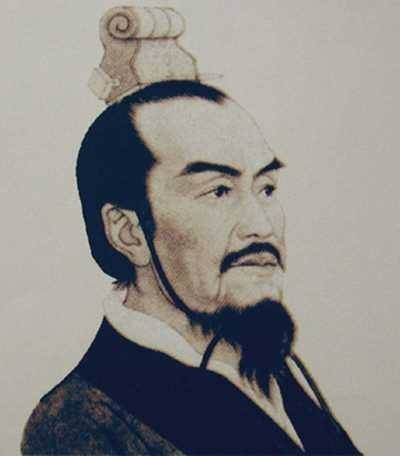
\includegraphics[width=0.3\textwidth]{pics/p003.jpg}
\vspace{-25pt}
\caption{李斯}
%\label{test}
\end{wrapfigure}

文/李碧華
\footnote{摘自《讀者》雜誌2018年9月號[言論1]與【讀者雜誌讀書會】臉書社團,圖:摘自網路}

26歲的李斯,是楚國一個看守糧倉的小文書。
糧囤附近有草葦圍住的糞坑。
李斯如廁時,見到枯瘦瑟縮又沾了糞的小耗子,
他想:人生如鼠啊,不在倉就在廁。
他不禁長歎:「一輩子有無出息,全看為自己找一個什麼位置。」

在一個月夜,他想,該換一種活法了。

清早,他匆匆離開家鄉、親人、沒前途的把老鼠腰斬的守倉員職位 $\cdots$ 這一走,
終其一生沒有再回去。他高升了。

很多年以後,他像當日殺鼠一樣,被判五刑加腰斬—劓刖、割舌、剁肢、笞殺同時執行之際便腰斬,最後慢慢碎屍。
一家老小、三族親戚、賓客門生 $\cdots$ 不分男女,一律斬首。
七八個劊子手斧起刀落,也是一直忙到傍晚,雨夜。雨整整下了一個月。

以上是錢寧作品{\Kai《秦相李斯》}中生死興衰的始末。

在辭典裡,再慘烈也不過占了幾句:「秦朝丞相,定郡縣制,開中國地方制度新局面。
為趙高誣陷謀反,腰斬於咸陽。」而腰斬,在中國古代酷刑中,也不過其中一項而已。

每一個人,當要過另一種生活時,必然也有另一種結局在等他。
這是當時的貨倉管理員上廁所時所料想不到的。
而斬殺他的指鹿為馬的趙高,亦逃不了「夷三族」的下場。

歷史便是這樣了。





    \backmatter

    \chapter{Appendix}
    Note that it the missing chapter number,  since it is behind
    the backmatter command.

    \FloatBarrier

    \begin{singlespacing}
        \printbibliography
    \end{singlespacing}

\end{document}

